\section{Presentazione degli obiettivi}
In questa breve trattazione, presenteremo l'implementazione di una semplice
chat in linguaggio Java, che sfrutta la crittografia asimmetrica per lo scambio dei
messaggi e l'invio di allegati. La chat realizzata possiede una GUI per l'interazione
con l'utente avente il seguente aspetto:
\begin{figure}[h]
\centering
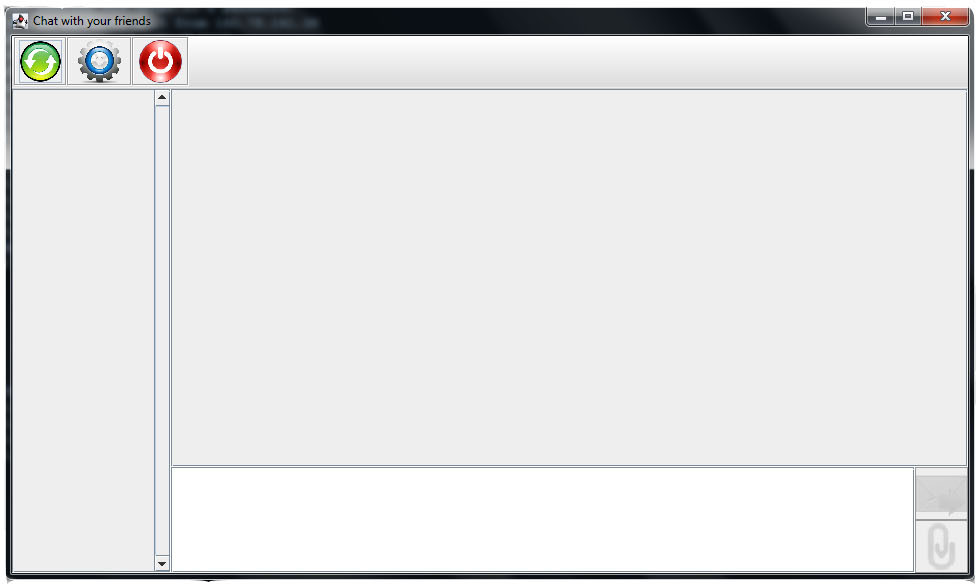
\includegraphics[scale=0.4]{gui1.jpg}
\end{figure}

Il riquadro in basso permette la scrittura di testo.
I due tasti laterali ad esso affiancati
consentono invece di inviare messaggi o allegati.
In alto sono presenti tre bottoni:
di essi, quello più a sinistra consente di scandire la rete per la ricerca di eventuali 
utenti che, in questo momento, stanno utilizzando la chat.
Tale scansione viene in ogni caso eseguita in automatico all'avvio del programma
e ripetuta periodicamente durante la sua esecuzione.
Quando un utente viene trovato, nel riquadro a sinistra 
dell'applicazione viene inserito un pulsante con il suo nickname.
Cliccandoci sopra, diventa possibile chattare con lui e inviargli messaggi.
Il bottone al centro, invece, gestisce le impostazioni,
mentre quello più a destra consente di chiudere l'applicazione.
La prima volta che il programma viene lanciato, inoltre,
compare una schermata di selezione del login:
\begin{figure}[h]
\centering
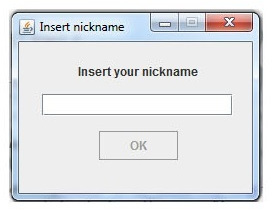
\includegraphics[scale=0.5]{login1.jpg}
\end{figure}

In questa scheda l'utente crea il proprio account, scegliendo un nickname da usare in chat
e vengono generate le chiavi pubblica e privata. Una volta digitato il nickname, il tasto
di conferma diventa cliccabile e ed è possibile iniziare ad usare l'applicazione.

In questa relazione, analizzeremo le varie classi della codifica proposta,
con particolare enfasi sul ruolo giocato da ognuna di esse.
Mostreremo, poi, i risultati ottenuti e, infine,
il funzionamento dell'intero programma qui presentato,
esponendo anche i test fatti in corso d'opera
in locale e sulla Virtual Private Network di ateneo.
Il lavoro svolto sarà, quindi, accompagnato dalle dovute conclusioni e
da un commento sui possibili sviluppi futuri.